\documentclass[10pt,twocolumn]{article}
\usepackage{float}
\usepackage[figurename=Fig., tablename=Tabla]{caption}
\setlength{\columnsep}{20.0pt}
\usepackage[a4paper, margin=22.5mm]{geometry}
\usepackage{amsmath}
\usepackage[utf8]{inputenc}
\usepackage{listings}
\usepackage{color}
\usepackage{graphicx}
\usepackage{caption}
\usepackage{subcaption}
\usepackage{mathtools}
\usepackage{enumerate}
\usepackage{multirow}
\usepackage{array}
\newcolumntype{L}[1]{>{\raggedright\let\newline\\\arraybackslash\hspace{0pt}}m{#1}}
\newcolumntype{C}[1]{>{\centering\let\newline\\\arraybackslash\hspace{0pt}}m{#1}}
\newcolumntype{R}[1]{>{\raggedleft\let\newline\\\arraybackslash\hspace{0pt}}m{#1}}
\title{Medición del campo el\'ectrico a partir de las curvas equipotenciales de una distrubuci\'on de carga}
\author{Gabriel Sandoval \\ gfsandovalv@unal.edu.co \and Sergio Cortéz \\sacortesc@unal.edu.co \and Juan Mojica \\jsmojicaj@unal.edu.co\\ \\Universidad Nacional de Colombia\\Facultad de Ciencias \\ Sede Bogotá}
\date{Febrero 2017}

\begin{document}
\maketitle{}
\begin{abstract}
The abstract goes here.
\end{abstract}

\section{Introducción}
La Introducción va aquí.
\section{Márco teórico}
El campo generado por una distribución de cargas estáticas, \emph{campo eléctrico}, es un campo conservativo, por lo que se puede ver como el gradiente de un potencial, como sigue. \cite{griffiths}
\begin{equation}\label{gradiente}
  \vec{E}=\vec{\nabla}V(\vec{r})
\end{equation}
El campo escalar $V(\vec{r})$ se conoce como \emph{potencial eléctrico}.\\
Si se conoce la forma funcional del potencial de la distribución, facilemte se obtiene el campo eléctrico de forma exacta. Sin embargo, si lo único conocido es la gráfica del potencial igualado a una cosntante $V(\vec{r})=V_0$, es decir las superficies equipotenciales (o curvas, en dos dimensiones), puede hacerse una apróximación númerica usando diferencias finitas en vez de infinitesimales.
\begin{equation*}
  \begin{split}
    \vec{\nabla}V(\vec{r})&=\Big(\dfrac{\partial}{\partial x}, \dfrac{\partial}{\partial y},
    \dfrac{\partial}{\partial z}\Big) V(\vec{r})\\
    &\approx \Big(\dfrac{\Delta}{\Delta x}, \dfrac{\Delta}{\Delta y}, \dfrac{\Delta}{\Delta z}\Big) V(\vec{r})\\
    &\approx \vec{E}(\vec{r})
  \end{split}
\end{equation*}
En particular, para una dimensión se tiene:
\begin{equation}\label{1dimension}
\vec{E}(\vec{r}) \approx \dfrac{\Delta V(x)}{\Delta x}=\dfrac{V_i-V_{i+1}}{x_i-x_{i+1}}  
\end{equation}
\section{Detalles experimentales}
Para \emph{dibujar} las líneas equipotenciales, se usó un tablero al que en su parte inferior se fija una placa recubierta con grafito, que además tiene un par de áreas recubiertas de un  material conductor, con alguna forma particular. Éstas se servirán como distribución de carga. Cada una de estas árear se conecta al estremo de una pila de 1.5V, de modo que la distrubución de carga, a gran escala, configura un dipolo. \\Además hay una especie de tenedor que sirve para moverse por el tablero, de modo que en la parte inferior haga contancto con la placa en el área recubierta con grafito y en la superior sirva como guía para trazar cada punto dela respectiva línea equipotencial. Al conectar este tenedor a un amperímetro y a una resistencia, se obtiene una medición. La idea es que el potencial generado por la distribución, en un punto, se compense con una caída de potencial dada por la resistencia de tal modo que la lectura en el amperímetro sea de 0.0 $\mu{}$A. En total se tienen siete  resistencias en serie, así el máximo de lineas equipotenciales que se pueden dibujar es de siete. \\
Las resistencias son iguales por lo que se espera una caída de potencial de $\frac{3}{14}$V por cada una. 

Se hallaron las curvas equipotenciales de tres distribuciones y, se escogieron aletoriamente tres puntos por cada distribución para hallar el campo tales puntos.

\section{Resultados y análisis}
Al realizar las curvas para cada distribución, se obtiene lo mostrado en la figura \ref{fig:curvas}.
\begin{figure}[H]
  \centering
  \begin{subfigure}[b]{0.80\linewidth}
    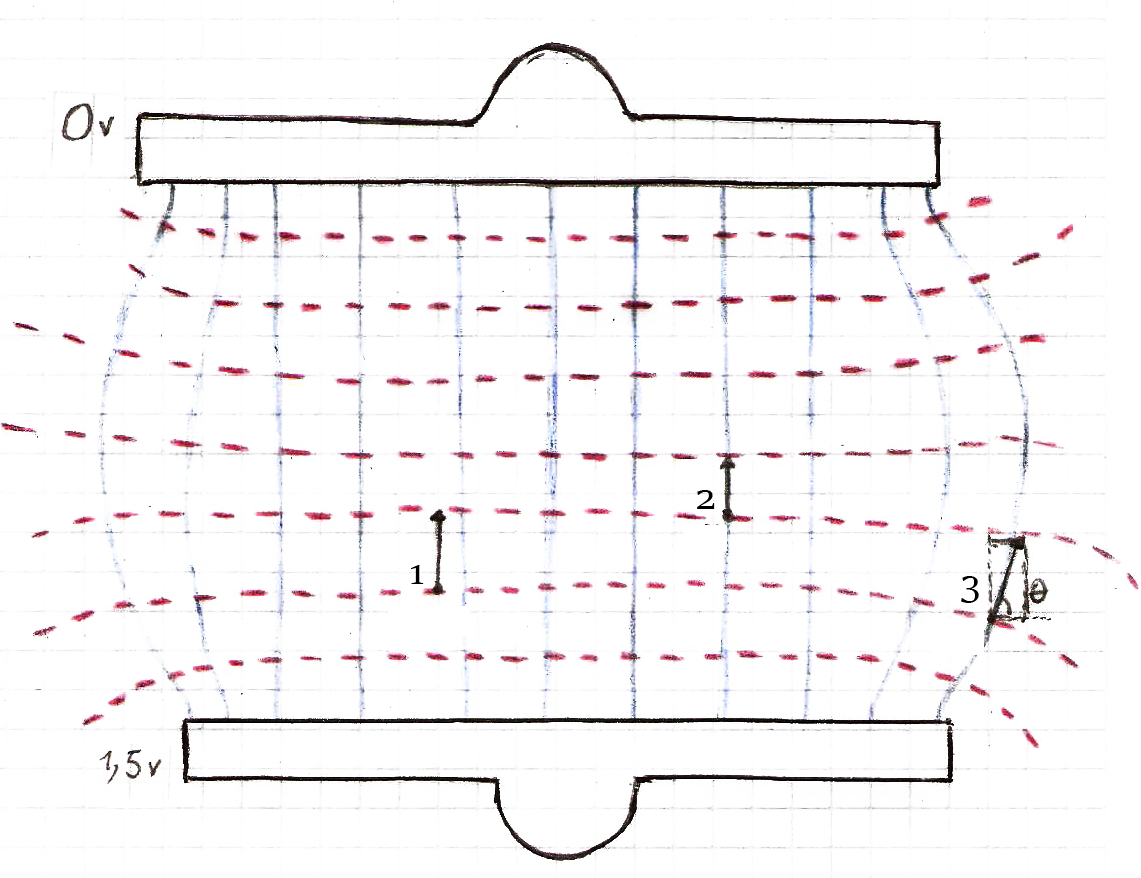
\includegraphics[width=\linewidth]{placas.png}
    \caption{Líneas Paralelas}
  \end{subfigure}
  
  \vspace{8mm}
    \begin{subfigure}[b]{0.80\linewidth}
    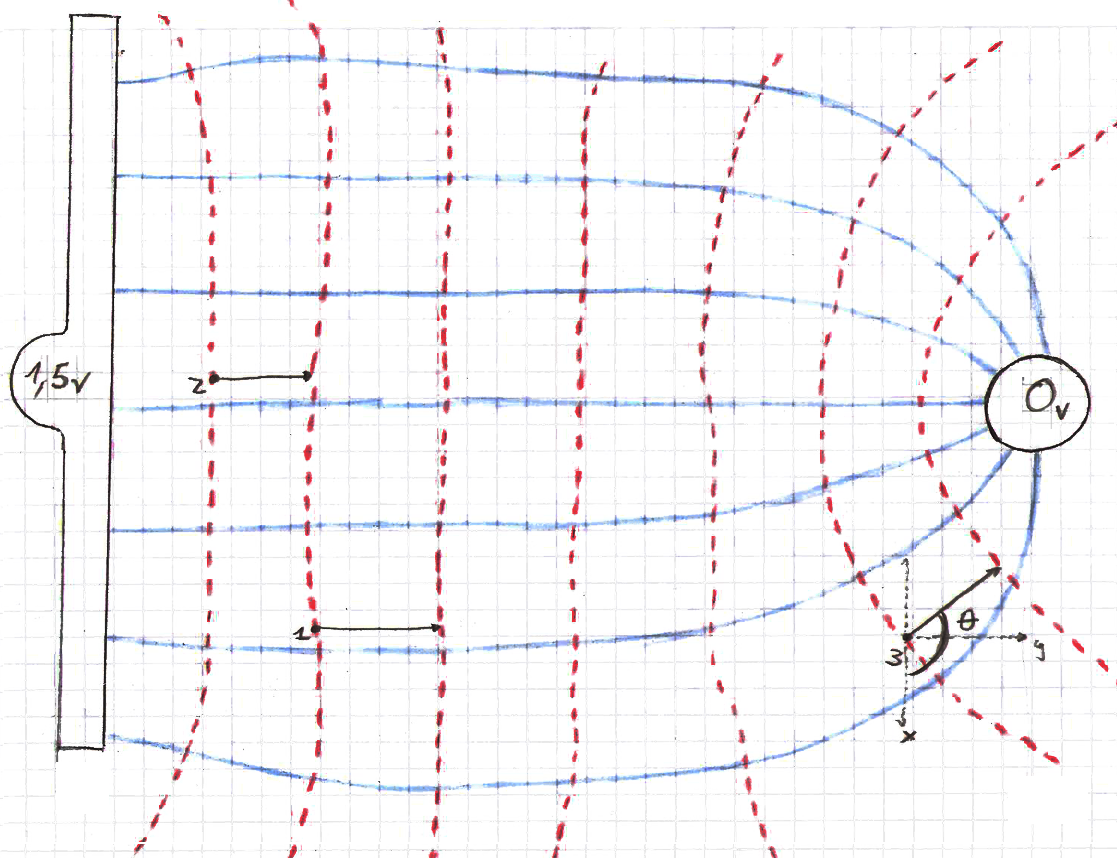
\includegraphics[width=\textwidth]{placa-esfera.png}
    \caption{Línea - Círculo}
  \end{subfigure}
  
  \vspace{8mm}
  \begin{subfigure}[b]{0.80\linewidth}
    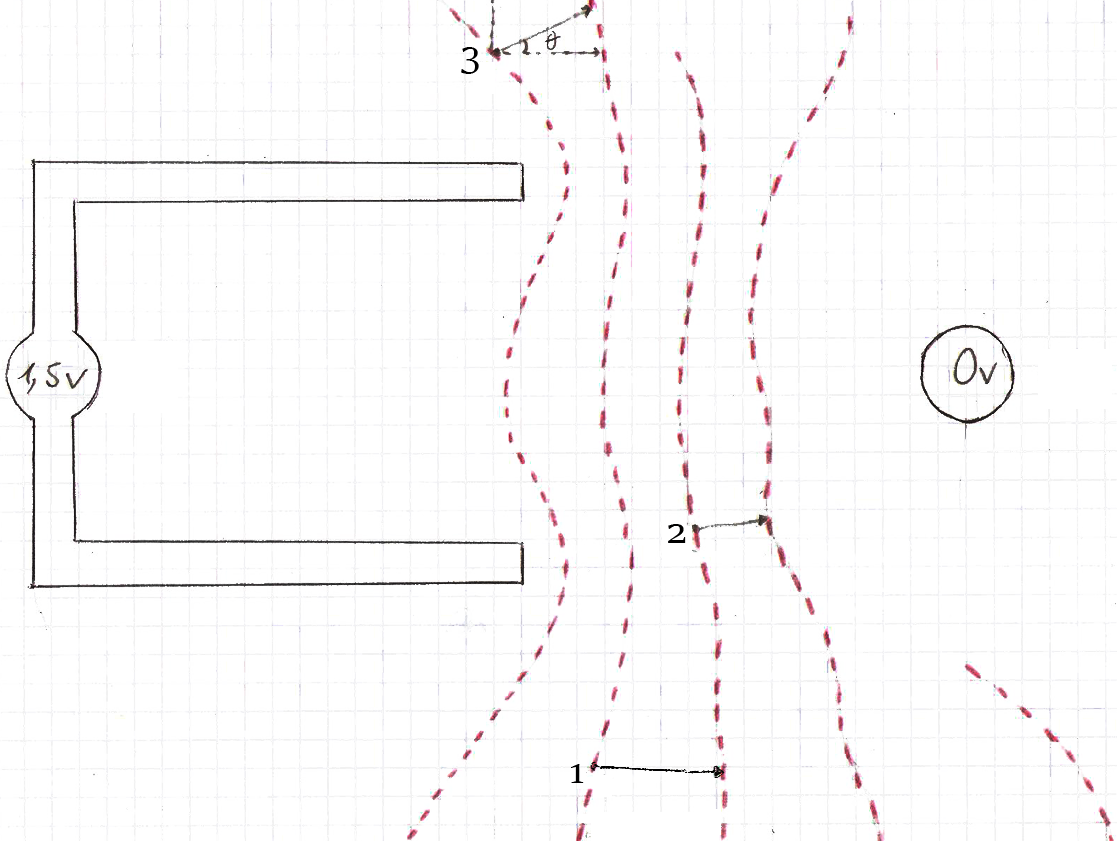
\includegraphics[width=\textwidth]{herradura_es.png}
    \caption{Herradura - Círculo}\label{fig:herradura}
  \end{subfigure}
  \caption{Curvas equipotenciales de tres distribuciones de carga}\label{fig:curvas}
\end{figure}
En la tercera distribución (Fig: \ref{fig:herradura}) no se completaron las curvas equipotenciales, ya que al pasar el sensor en la zona zona cercana al cero (polaridad negativa), las mediciones del amperímetro cambiaba drásticamente de negativo a positivo, y resultó complicado marcar los puntos.\\

  Lo que sigue para determinar el campo eléctrico en los puntos escogidos, es medir la distancia entre la línea sobre la que se situó el punto, y la siguiente, acercándose a la polaridad negativa (donde el voltage es nulo); y conocer la diferencia de potencial entre estas líneas (véase Tabla \ref{tab:campo1}).

    \begin{table}
      \scalebox{0.95}{
        \begin{tabular}{ |c|C{1.6cm}|c|C{2.4cm}| }
        \hline
        \rule{0pt}{18pt}
        Pt. \# & \begin{tabular}{c} $\Delta x$ \\($10^{-2}$ m)\end{tabular}   & $\Delta V$ (V) & \begin{tabular}{c} $\vert \vec{E}\vert$ \\(V$\cdot 10^{-2}$ m$^{-1}$)\end{tabular}
        \\ \hline
        \multicolumn{4}{ |c| }{Líneas paralelas}\\
        \hline
        1 & 0.9 & 0.21 & 0.23 \\ 
        2 & 0.8 & 0.21 & 0.26 \\ 
        3 & 1.2 & 0.21 & 0.17 \\
        \hline
        \multicolumn{4}{ |c| }{Línea - Círculo}\\
        \hline
        1 & 2.3 & 0.21 & 0.23 \\ 
        2 & 1.8 & 0.21 & 0.26 \\ 
        3 & 2.2 & 0.21 & 0.17 \\
        \hline
        \multicolumn{4}{ |c| }{Herradura - Círculo}\\
        \hline
        1 & 2.0 & 0.21 & 0.23 \\ 
        2 & 1.3 & 0.21 & 0.26 \\ 
        3 & 2.5 & 0.21 & 0.17 \\
        \hline
      \end{tabular}}
      \caption{aproximación del campo eléctrico en algunos putos de cada distribución}\label{tab:campo1}
    \end{table}

  Para darle el carácter vectorial al campo debe definirse un sistema de referencia en cada \emph{dibujo}. Por simplicidad se escogió el sistema de coordenadas polares. En la tabla \ref{tab:vectores} se muestra la magnitud y argumento de cada vector.

  \begin{center}
    \begin{table}[H]
      \begin{tabular}{ |c| c| c| }
        \hline
        \multirow{2}{*}{Punto \#} \rule{0pt}{15pt}& \multicolumn{2}{ c| }{$\vec{E}$} \\
        \cline{2-3}
        \rule{0pt}{16pt}
     &  $\vert \vec{E}\vert$ (V$\cdot 10^{-2}$ m$^{-1}$) & $ \arg{\vec{(E)}}$ (rad)\\ \hline
        \multicolumn{3}{ |c| }{Líneas paralelas}\\
        \hline
        1 & 0.23 & 1.57  \\ 
        2 & 0.26 & 1.57  \\ 
        3 & 0.17 & 0.73 \\
        \hline
        \multicolumn{3}{ |c| }{Línea - Círculo}\\
        \hline
        1 & 0.23 & 0.0 \\ 
        2 & 0.26 & 0.0 \\ 
        3 & 0.17 & 0.67\\
        \hline
        \multicolumn{3}{ |c| }{Herradura - Círculo}\\
        \hline
        1 & 0.23 & -0.30\\ 
        2 & 0.26 & 0.24\\ 
        3 & 0.17 & 0.16\\
        \hline
      \end{tabular}
      \caption{Magnitud y argumento de $\vec{E}$ para cada distribución}\label{tab:vectores}
    \end{table}
  \end{center}

  
\section{Conclusiones}
\begin{itemize}
\item No es necesario conocer una expresión analítica que describa las curvas equipotenciales de una distribución de carga, sino que se puede aproximar realizando mediciones de distancia y potencial.
\item La forma de las curvas equipotenciales depende de la forma geométrica de las distribución en cuestión.
\end{itemize}
\begin{thebibliography}{1}
  \bibitem{griffiths} David J. Griffiths {\em Introduction to Electrodynamics} Third Edition,  1999. Prentice Hall.
  \end{thebibliography}
\end{document}
